% Created by tikzDevice version 0.10.1 on 2017-11-26 21:02:59
% !TEX encoding = UTF-8 Unicode
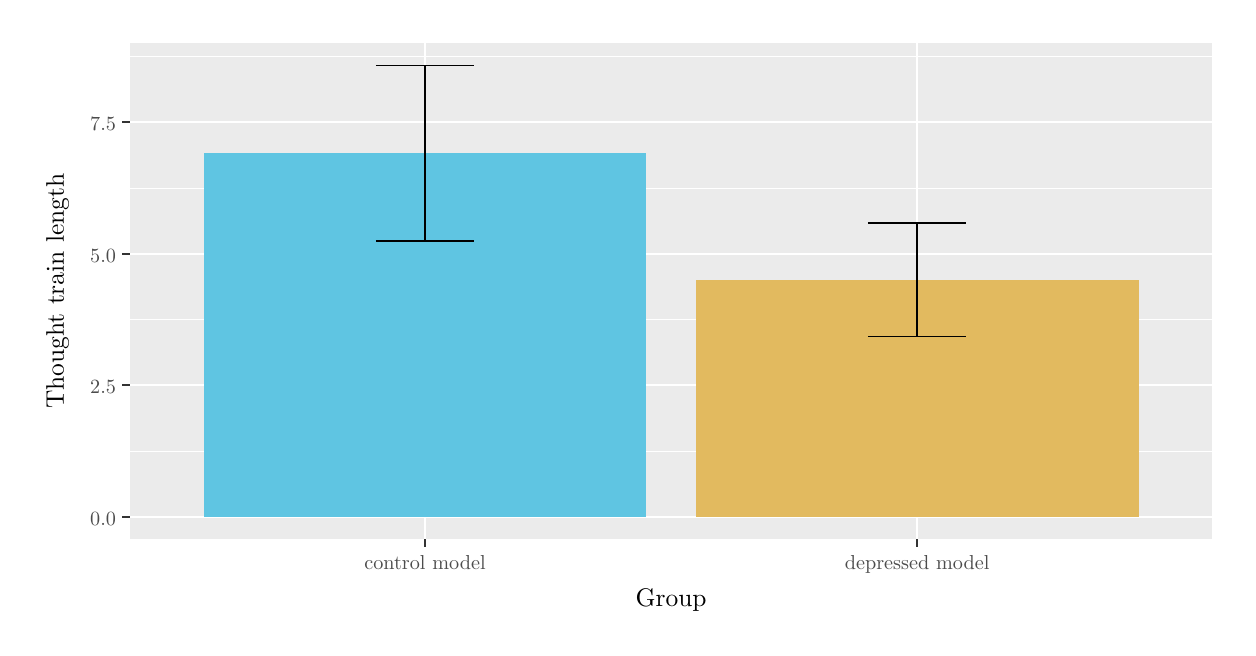
\begin{tikzpicture}[x=1pt,y=1pt]
\definecolor{fillColor}{RGB}{255,255,255}
\path[use as bounding box,fill=fillColor,fill opacity=0.00] (0,0) rectangle (433.62,216.81);
\begin{scope}
\path[clip] (  0.00,  0.00) rectangle (433.62,216.81);
\definecolor{drawColor}{RGB}{255,255,255}
\definecolor{fillColor}{RGB}{255,255,255}

\path[draw=drawColor,line width= 0.6pt,line join=round,line cap=round,fill=fillColor] (  0.00,  0.00) rectangle (433.62,216.81);
\end{scope}
\begin{scope}
\path[clip] ( 36.87, 31.92) rectangle (428.12,211.31);
\definecolor{fillColor}{gray}{0.92}

\path[fill=fillColor] ( 36.87, 31.92) rectangle (428.12,211.31);
\definecolor{drawColor}{RGB}{255,255,255}

\path[draw=drawColor,line width= 0.3pt,line join=round] ( 36.87, 63.84) --
	(428.12, 63.84);

\path[draw=drawColor,line width= 0.3pt,line join=round] ( 36.87,111.36) --
	(428.12,111.36);

\path[draw=drawColor,line width= 0.3pt,line join=round] ( 36.87,158.89) --
	(428.12,158.89);

\path[draw=drawColor,line width= 0.3pt,line join=round] ( 36.87,206.42) --
	(428.12,206.42);

\path[draw=drawColor,line width= 0.6pt,line join=round] ( 36.87, 40.07) --
	(428.12, 40.07);

\path[draw=drawColor,line width= 0.6pt,line join=round] ( 36.87, 87.60) --
	(428.12, 87.60);

\path[draw=drawColor,line width= 0.6pt,line join=round] ( 36.87,135.13) --
	(428.12,135.13);

\path[draw=drawColor,line width= 0.6pt,line join=round] ( 36.87,182.65) --
	(428.12,182.65);

\path[draw=drawColor,line width= 0.6pt,line join=round] (143.57, 31.92) --
	(143.57,211.31);

\path[draw=drawColor,line width= 0.6pt,line join=round] (321.41, 31.92) --
	(321.41,211.31);
\definecolor{fillColor}{RGB}{95,197,226}

\path[fill=fillColor] ( 63.54, 40.07) rectangle (223.60,171.40);
\definecolor{fillColor}{RGB}{226,186,95}

\path[fill=fillColor] (241.39, 40.07) rectangle (401.44,125.70);
\definecolor{drawColor}{RGB}{0,0,0}

\path[draw=drawColor,line width= 0.6pt,line join=round] (125.79,203.16) --
	(161.36,203.16);

\path[draw=drawColor,line width= 0.6pt,line join=round] (143.57,203.16) --
	(143.57,139.65);

\path[draw=drawColor,line width= 0.6pt,line join=round] (125.79,139.65) --
	(161.36,139.65);

\path[draw=drawColor,line width= 0.6pt,line join=round] (303.63,146.19) --
	(339.20,146.19);

\path[draw=drawColor,line width= 0.6pt,line join=round] (321.41,146.19) --
	(321.41,105.22);

\path[draw=drawColor,line width= 0.6pt,line join=round] (303.63,105.22) --
	(339.20,105.22);
\end{scope}
\begin{scope}
\path[clip] (  0.00,  0.00) rectangle (433.62,216.81);
\definecolor{drawColor}{gray}{0.30}

\node[text=drawColor,anchor=base east,inner sep=0pt, outer sep=0pt, scale=  0.73] at ( 31.92, 37.04) {0.0};

\node[text=drawColor,anchor=base east,inner sep=0pt, outer sep=0pt, scale=  0.73] at ( 31.92, 84.57) {2.5};

\node[text=drawColor,anchor=base east,inner sep=0pt, outer sep=0pt, scale=  0.73] at ( 31.92,132.10) {5.0};

\node[text=drawColor,anchor=base east,inner sep=0pt, outer sep=0pt, scale=  0.73] at ( 31.92,179.62) {7.5};
\end{scope}
\begin{scope}
\path[clip] (  0.00,  0.00) rectangle (433.62,216.81);
\definecolor{drawColor}{gray}{0.20}

\path[draw=drawColor,line width= 0.6pt,line join=round] ( 34.12, 40.07) --
	( 36.87, 40.07);

\path[draw=drawColor,line width= 0.6pt,line join=round] ( 34.12, 87.60) --
	( 36.87, 87.60);

\path[draw=drawColor,line width= 0.6pt,line join=round] ( 34.12,135.13) --
	( 36.87,135.13);

\path[draw=drawColor,line width= 0.6pt,line join=round] ( 34.12,182.65) --
	( 36.87,182.65);
\end{scope}
\begin{scope}
\path[clip] (  0.00,  0.00) rectangle (433.62,216.81);
\definecolor{drawColor}{gray}{0.20}

\path[draw=drawColor,line width= 0.6pt,line join=round] (143.57, 29.17) --
	(143.57, 31.92);

\path[draw=drawColor,line width= 0.6pt,line join=round] (321.41, 29.17) --
	(321.41, 31.92);
\end{scope}
\begin{scope}
\path[clip] (  0.00,  0.00) rectangle (433.62,216.81);
\definecolor{drawColor}{gray}{0.30}

\node[text=drawColor,anchor=base,inner sep=0pt, outer sep=0pt, scale=  0.73] at (143.57, 20.91) {control model};

\node[text=drawColor,anchor=base,inner sep=0pt, outer sep=0pt, scale=  0.73] at (321.41, 20.91) {depressed model};
\end{scope}
\begin{scope}
\path[clip] (  0.00,  0.00) rectangle (433.62,216.81);
\definecolor{drawColor}{RGB}{0,0,0}

\node[text=drawColor,anchor=base,inner sep=0pt, outer sep=0pt, scale=  0.92] at (232.49,  7.83) {Group};
\end{scope}
\begin{scope}
\path[clip] (  0.00,  0.00) rectangle (433.62,216.81);
\definecolor{drawColor}{RGB}{0,0,0}

\node[text=drawColor,rotate= 90.00,anchor=base,inner sep=0pt, outer sep=0pt, scale=  0.92] at ( 13.08,121.61) {Thought train length};
\end{scope}
\end{tikzpicture}
